\documentclass{article}


\usepackage{authblk}
\usepackage{listings, chngcntr}
\usepackage{textcomp}
\usepackage{float}
\usepackage[T1]{fontenc}
\usepackage{indentfirst}
\usepackage{graphicx}
\usepackage{array}
\usepackage{caption} 
\usepackage{hyperref}
\usepackage{verbatim}
\usepackage{float}
\usepackage{subcaption}
\usepackage{gensymb}
\usepackage{amsmath}
\usepackage{geometry}
\usepackage{multirow}

\geometry{
    a4paper,
    left=30mm,
    right=30mm,
    top=30mm,
    bottom=40mm
}

\begin{document}

\title{Lock In Amplifier and Hall effect}
\author[1]{Woojin Han}
\affil[1]{Seoul National University, Seoul 151-747, Korea}
\maketitle

\begin{abstract}
    In this experiment, the signal processing modules are measured and tested.
    The python module \verb|lock_in_data| is made and uploaded which helps to read image files from the oscilloscope and organize to plot easily.
    The lock-in amplifier circuit is improved in the phase shift measurement, and the higher accuracy of signal processing is performed.
    The two input in the double-balanced mixer is also plotted in the oscilloscope, to measure the phase difference directly.
    In this method, the gain in phase plot and the lock-in amplifier results have a low measurement error of $0.1 [mV]$
    The short-range peak nature of the preamplifier module is claimed and the log scale plot is provided.
    Therefore, the magnetic dipole moment density of the magnet is accurately measured in $M = (3.3 \pm 0.1) \times 10^{16} [A/m]$, highly improved than seniority results.
\end{abstract}

\section{Introduction}
 The electric signals have unavoidable noise and offsets.
 By now, many apparatus gives electric outputs which are not free from these restraints.
 Therefore signal processing like a lock-in amplifier is important.
 In this report, the Lock-in amplifier and its module are experimented with different signal frequencies and conditions.
 But, the lock-in detection had critical issues in phase measurement.
 I improved the circuit to directly measure the phase difference. \ref{methods: start}
 Also, I make the python module that can help analysis in lock-in amplifier and other experiments, explained in \ref{intro: python_module} and uploaded in \cite{github}.
 Finally, the detection is used to measure the magnetic dipole moment by the hall sensor.

\subsection{Lock In detection}
\label{intro: lock_in_detection}
 Lock-in detection is the experiment to measure the subtle signal distinct to a noise or a direct current(DC) offset.
 Mostly the lock-in detection uses Double Balance Mixer(DBM) circuit.
 DBM circuit is shown schematical in Fig. \ref{fig: DBM_intro}.
 The circuit has two inputs, the signal input($V_{in}$) and the reference input($V_{ref}$).
 By the diodes in the circuit, the output voltage only depends on the sign of the reference input.
 In each, the output of this circuit is $V_{in} \times sgn(V_{ref})$ for $sgn$ a sign function.

 \begin{figure}[H]
  \centering
  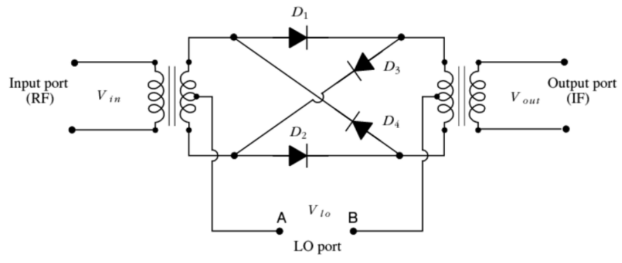
\includegraphics[width=7cm]{../results/DBM_intro_circuit.png}
  \caption{The abstract circuit of DBM, adapted by \cite{manual}}
  \label{fig: DBM_intro}
 \end{figure}

 Then, the output signal passes the low-pass filter.
 The low-pass filter is formed in resistance and capacitor to only filter out the low-frequency signal.
 The filtering bandwidth is the parameter of the frequency area that can only pass by.
 For a sufficiently good low-pass filter, the filtered signal can be used as the DC signal.
 To explain the lock-in amplifier circuit, two cases can be exampled.
 If the reference input has a different frequency than the signal input in the DBM circuit, the output results do not have periodicity.
 The low-pass filter can be expected to make the signal in DC, it performs to average the input signal in time.
 Therefore, the signal of different frequencies vanishes in the output of the low-pass filter.
 The term different is calculated near the filtering bandwidth, by the definition.
 If the reference input and the signal have the same frequency, the signal input does not vanish by the low-pass filter.
 In each, the DC output from the low-pass filter is given by $V_0 \cos \phi$, $V_0$ is the signal input and $\phi$ is the phase difference between two signals.
 So, the absolute amplitude of the output signal takes its maximum in phase difference $0, 180 \degree$.


\subsection{Data Analysis Module}
\label{intro: python_module}
 While performing a Lock-In experiment, detected oscilloscope results can be returned in the form of \textbf{.csv} or \textbf{.png} files.
 However, there are too many time points in each \textbf{.csv} file, it is recommended to read the oscilloscope screen for each detection.
 Also, each experiment has various parameters controlled by each panel so the modification of each data takes complicated forms.
 Therefore, I build a clean module for a Lock-In experiment result analysis that can help the successor in two big ways.

 First, it supports \verb|lock_in_data| type and \verb|read_png()| method so that helps to read \textbf{.png} file fast.
 To run this module, we need a labeled Excel file that informs the parameters and the picture name.
 For example, let the preamplifier experiment of gain 2, input signal frequency of $50  [kHz]$ be saved by the file name "TEK000056.png".
 Then the labeled Excel file should contain a row 2, 50, and 56.
 And also the column of the picture name should be "name".
 We must modify the \verb|get_data_labels()|, which is the detected value of the oscilloscope \textbf{.png} for each experiment.
 I assumed that each experiment is placed in a different sheet of Excel file.
 
 \begin{verbatim}
reading 183 out of 701
Commit data: 1960
Commit data: 208
Commit data: 45.72
Commit data: -45.58
1_amplitude : 1960
2_amplitude : 208
12_phase : 45.72
21_phase : -45.58
{'gain': 10.0, 'frequency(kHz)': 200}
 \end{verbatim}
 

 By running \verb|main.py|, the example output above prints out.
 The module crops the exact position of the oscilloscope screenshots in \verb|./ERROR.PNG|, the only work to do is to read the number in the image.
 The commission of data is grouped simultaneously in \verb|lock_in_data| type and saved by \verb|datum. pkl|.
 The \verb|datum| is a dictionary that contains each experiment and data conveniently.
 For example, \verb|datum['preamplifier'][0]| is data collected in the preamplifier circuit the first time.

 Second, this module makes the plotting even more convenient.
 The Lock-In experiment needs to control some parameters and only plots a graph with selected parameters and results.
 Therefore, there must be a repeated structure of a plotting code scheme, which is very uncomfortable and crummy.
 In \verb|lock_in_data.py| header have the method of \verb|phys_plot()| which supports the faster way to plot a list of \verb|lock_in_data| type.
 For example, the code following plots the ratio of \verb|data. results[0]| and \verb|data. results[1]| in the function of signal frequency, only for the gain parameter set by 1.

 \begin{verbatim}
    fig = lock_in_data.phys_plot(
        datum[experiment],
        'frequency(kHz)',
        lambda x : x.results[0]/x.results[1], 
        {'gain': 1},
        x_label="frequency [kHz]",
        y_label= "Amplitude_ratio",
        fmt = 'ko'
        )    
 \end{verbatim}

 Every code and raw data is uploaded in \cite{github}, it is complete by itself so that only running \verb|main.py| will help the successor to use this module.
 For window system users must change the \verb|./| to \verb|.\\| to detour compatibility.

\section{Methods}
\label{methods: start}
Apparatus: Signal Processor (\cite{signal_processor}), oscilloscope, function generator, MG910 Hall ellement(\cite{hall_sensor})
The Lock-In module has been set up in the intermediate physics experiment laboratory, at Seoul National University.
The signal processor from Teach Spin is modular architecture with multiple circuits such as a preamplifier, and low pass amplifier.
I subtly improve the experimental method, especially the circuit modification, to specify the phase difference between the signal and reference input.
Every result of each experiment is in \ref{results: start} with the same subsection name.

\subsection{Preamplifier}
 The preamplifier circuit is not modified.
 Fig. \ref{fig: preamplifier_circuit}(a) shows the preamplifier circuit I used.
 Fig. \ref{fig: preamplifier_circuit}(b) is one of the raw data results while performing the circuit.

 \begin{figure}[ht]
  \centering
  \begin{subfigure}[b]{7cm}
      \centering
      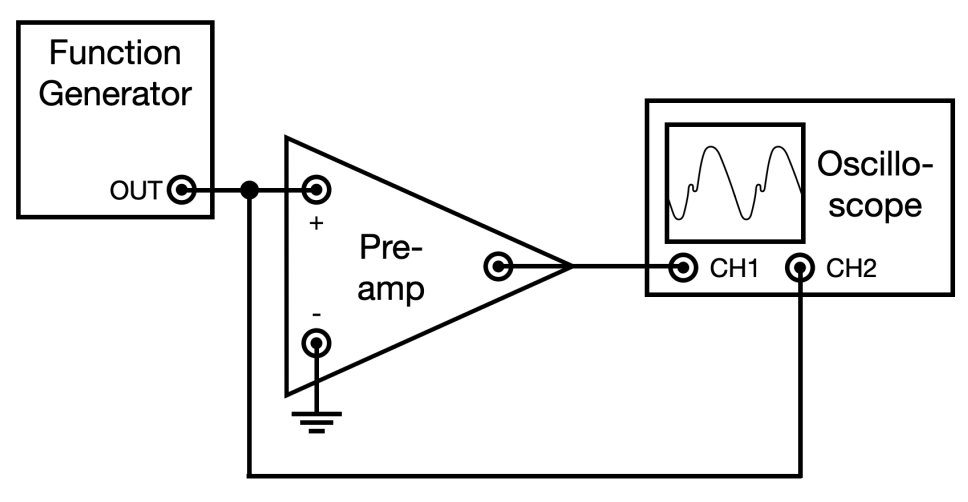
\includegraphics[width=7cm]{../results/preamplifier_circuit.png}
      \caption{}
  \end{subfigure}
  \hfill
  \begin{subfigure}[b]{7cm}
      \centering
      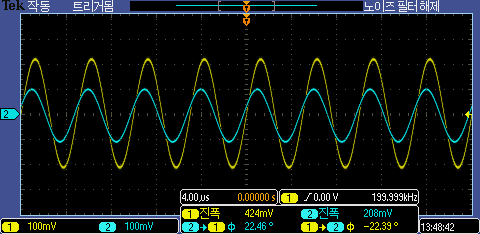
\includegraphics[width=7cm]{../raw_data/TEK00071.PNG}
      \caption{}
  \end{subfigure}
  \hfill
  \caption{Schematic diagram of (a) preamplifier circuit, adapted form  \cite{signal_processor}.
  (b)The oscilloscope screen capture of frequency 200 $kHz$ and gain$=2$.
  The blue line is the reference input and the yellow line is the signal output.}
  \label{fig: preamplifier_circuit}
\end{figure}
 I measured 57 different frequencies in each gain 1, 2, 5, 10, 20.
\subsection{Phase Shifter: Lagging phase detection}
The phase shifter provided in the signal processor is not uniformly performing, so the shifted phase is dependent on input signal frequency.
I define the word lagged phase as the difference between the real shifted phase and the displayed phase shift.
The manual suggests using the linear regression results of this measurement to complement the lagged phase, but as \ref{results: phase shifter} shows that the shifted phase amount is too big to cause errors.
Therefore I use three channels in the oscilloscope at the base of this circuit.
The first two of them are a reference and the phase-shifted signal just like this experiment circuit.
And the last one is set to the final signal of each experiment.
I have emphasized the modified circuit in each subsection.
\begin{figure}[ht]
    \centering
    \begin{subfigure}[b]{7cm}
        \centering
        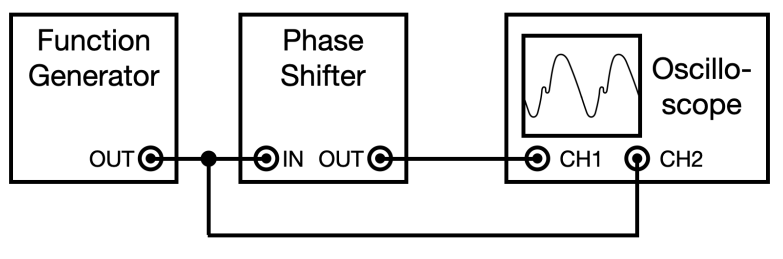
\includegraphics[width=7cm]{../results/phase_shifter_circuit.png}
        \caption{}
    \end{subfigure}
    \hfill
    \begin{subfigure}[b]{7cm}
        \centering
        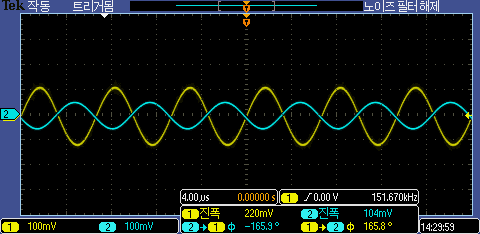
\includegraphics[width=7cm]{../raw_data/TEK00306.PNG}
        \caption{}
    \end{subfigure}
    \hfill
    \caption{Schematic diagram of (a) phase shifter circuit, adapted form  \cite{signal_processor}.
    (b)The oscilloscope screen capture of frequency 150 $Hz$ and $\pi/2$ phase shifted.
    The blue line is the reference input and the yellow line is the signal output.}
    \label{fig: phase_shifter_circuit}
  \end{figure}

 Fig. \ref{fig: phase_shifter_circuit}(b) shows the exact lagged phase in the module.
 The phase shifted amount displayed on the signal processor is $\pi/2$ but its real shifted phase is about $\pi$.
 I measured 17 different frequencies in each displayed phase shift value.

 \subsection{Lock In detection: DBM}
 The Lock-In detection is implemented by Double Balanced Mixer(DBM) explained at \ref{intro: lock_in_detection}.
 In this experiment, the DBM performance is checked.
 However, the lagged phase induced by the phase shifter and preamplifier huts the accurate measurement of the following experiments,
 I also display the phase-shifted input signal of the DBM module in the third channel of the oscilloscope.
 \begin{figure}[ht]
    \centering
    \begin{subfigure}[b]{7cm}
        \centering
        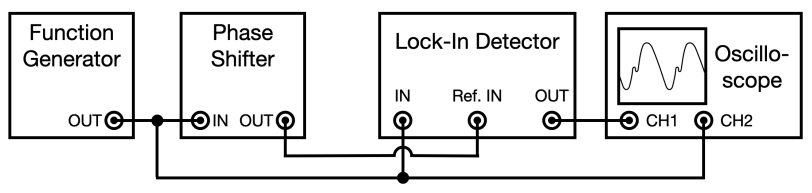
\includegraphics[width=7cm]{../results/DBM_circuit.png}
        \caption{}
    \end{subfigure}
    \hfill
    \begin{subfigure}[b]{7cm}
        \centering
        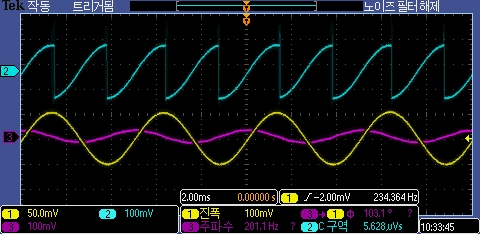
\includegraphics[width=7cm]{../raw_data/TEK00396.PNG}
        \caption{}
    \end{subfigure}
    \hfill
    \caption{Schematic diagram of (a) DBM circuit, adapted form  \cite{signal_processor}.
    (b)The oscilloscope screen capture of frequency 200 $Hz$ and $\pi/2$ phase shifted.
    The yellow line is the reference input and the purple line is the phase-shifted input.
    The blue line is the DBM output which performs well.
    }
    \label{fig: DBM_circuit}
  \end{figure}
 Fig. \ref{fig: DBM_circuit}(a) is the manual circuit arrangement, which has an inevitable error by the lagged phase.
 But by the subtle line connection, we can display the exact phase shit in the oscilloscope and can measure the real shift phase.
 So in the rest of the experiments, I modulate the phase difference by the measured value displayed in the oscilloscope.
 Fig. \ref{fig: DBM_circuit}(b) is the example results of the DBM experiment.
 It is definite to claim the phase difference between two input waves is $\pi/2$.
 But by the unavoidable error, the phase difference value fluctuates about $5\degree$, I read the median value while experimenting.
 I measured 21 different frequencies in each phase shift value of 0, $\pi/2$, $\pi$, and $3\pi/2$.

\subsection{Low-Pass Amplifier}
 The direct current offset is filtered by the low-pass amplifier.
 The amplifier has three parameters of $dB/oct$ and the time constant of the RC circuit.

 \begin{figure}[ht]
    \centering
    \begin{subfigure}[b]{7cm}
        \centering
        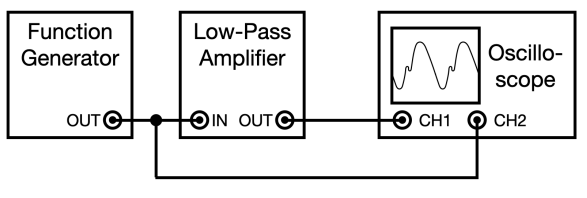
\includegraphics[width=7cm]{../results/low_pass_amplifier_circuit.png}
        \caption{}
    \end{subfigure}
    \hfill
    \begin{subfigure}[b]{7cm}
        \centering
        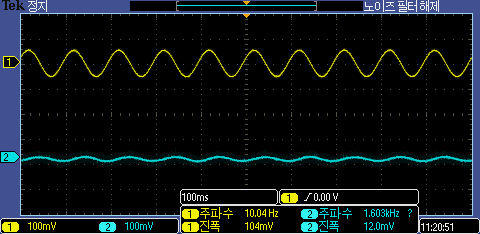
\includegraphics[width=7cm]{../raw_data/TEK00453.PNG}
        \caption{}
    \end{subfigure}
    \hfill
    \caption{Schematic diagram of (a) low pass amplifier circuit, adapted form  \cite{signal_processor}.
    (b)The oscilloscope screen capture of frequency 10 $Hz$ and $6 dB/oct$, the time constant of 0.1 s.
    The yellow line is the reference input and the blue line is the low-pass amplifier output which performs well.
    }
    \label{fig: low_pass_amplifier_circuit}
  \end{figure}

 Since it is applied to filter the high-frequency signals, in order of time constants, I have measured the signal for $0.1Hz$ to $50Hz$.
 The 10Hz result is even undetectable, as Fig. \ref{fig: low_pass_amplifier_circuit}(b) shows.
 Also widely broaden bandlike signal is observed, which is detailed in \ref{results: low pass filter}

 \subsection{Lock-In Amplifier: Noise detection}
 There are two steps in the noise detection experiment.
 The first is to check whether the noise provided by the signal processor is qualified by Fast Fourier Transform (FFT) included in the oscilloscope.
 The second is to form a Lock-In detection experiment to figure out a signal from the noise.
 \begin{figure}[ht]
    \centering
    \begin{subfigure}[b]{7cm}
        \centering
        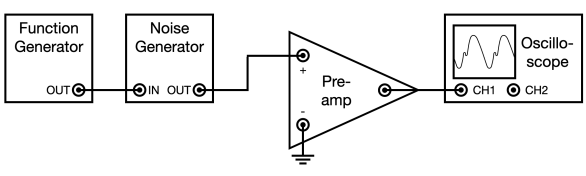
\includegraphics[width=7cm]{../results/noise_circuit.png}
        \caption{}
    \end{subfigure}
    \hfill
    \begin{subfigure}[b]{7cm}
        \centering
        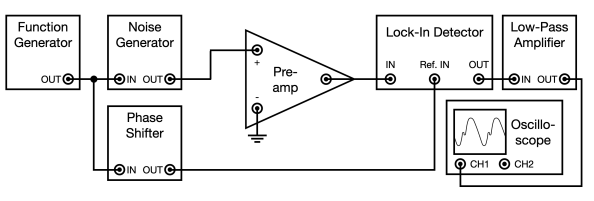
\includegraphics[width=7cm]{../results/noise_detection_circuit.png}
        \caption{}
    \end{subfigure}
    \hfill
    \caption{Schematic diagram of (a) noise generator and (b)the noise detection circuit, adapted form  \cite{signal_processor}.}
    \label{fig: noise detection}
  \end{figure}
 Fig. \ref{fig: noise detection}(a) shows the circuit of the first step.
 I put one plain channel to emphasize the noise signal with the unperturbed one.
 Fig. \ref{fig: noise detection}(b) represents the circuit of the second step.
 In this case, I plot a gain in the function of phase difference which must be measured precisely so that can give reliability to a regression.
 Therefore, I put two more channels in the oscilloscope, a reference and the noise signal each.
 The raw data of this experiment is plotted \ref{results: noise detection}.

\subsection{Lock-In detection: DC offset stability}
 To find a drift slope of a DC offset, the experiment is performed by the following circuit.
 Also, in this experiment the phase difference is fixed up to $\pi$, the circuit contains two more channels of reference and phase-shifted reference signal.
 \begin{figure}[H]
    \centering
    \begin{subfigure}[b]{7cm}
        \centering
        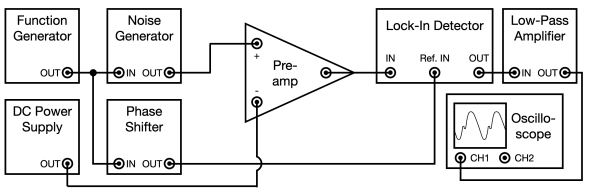
\includegraphics[width=7cm]{../results/DC_off_set_circuit.png}
        \caption{}
    \end{subfigure}
    \hfill
    \begin{subfigure}[b]{7cm}
        \centering
        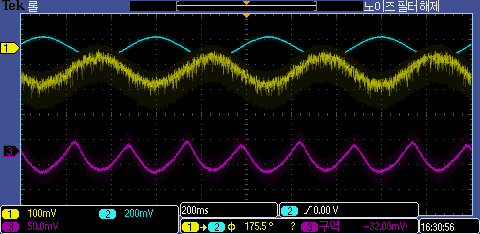
\includegraphics[width=7cm]{../raw_data/TEK00640.PNG}
        \caption{}
    \end{subfigure}
    \hfill
    \caption{Schematic diagram of (a) Lock-In DC offset stability measure circuit, adapted form  \cite{signal_processor}.
    (b)The oscilloscope screen capture of frequency 2 $Hz$ and $12 dB/oct$, the time constant of $0.03$ s the phase shifted value is $\pi$ the noise is added amount of $10^{-2}$.
    The blue line is the phase-shifted reference input and the yellow line is the noise-added signal.
    The purple line is the DBM Lock-In results.
    }
    \label{fig: DC_off_set_circuit}
  \end{figure}
 Fig. \ref{fig: DC_off_set_circuit}(a) is the circuit of the experiment.
 I used signal splitters in the Lock-In detector input and output to directly measure the phase difference between two inputs.
 Therefore, it can be very precisely controlled in this experiment, I have measured the gain from 25 different amounts of DC offset fixing phase difference in $\pi$.

 \subsection{Lock-In detection: Hall effect}
 The hall element signal is small so that the noise dominates the signal.
 Therefore, the frequency fixed Lock-In detection helps the signal distinguishable.
 The circuit is formed as the manual, but the phase difference is also directly measured as above experiments.
 \begin{figure}[ht]
    \centering
    \begin{subfigure}[b]{7cm}
        \centering
        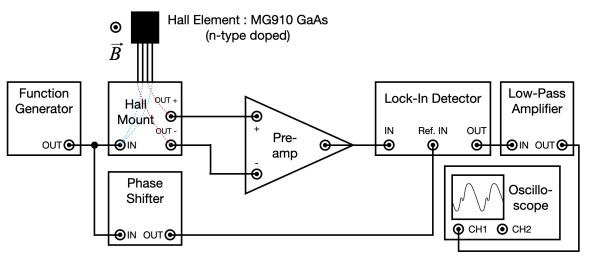
\includegraphics[width=7cm]{../results/hall_sensor_circuit.png}
        \caption{}
    \end{subfigure}
    \hfill
    \begin{subfigure}[b]{7cm}
        \centering
        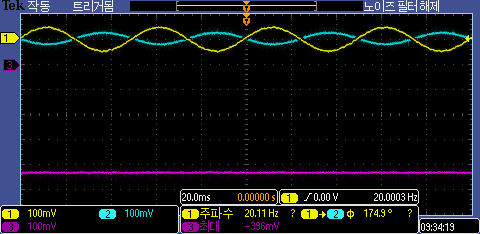
\includegraphics[width=7cm]{../raw_data/TEK00697.PNG}
        \caption{}
    \end{subfigure}
    \hfill
    \caption{Schematic diagram of (a) Hall element experiment circuit, adapted form  \cite{manual}.
    (b)The oscilloscope screen capture of frequency 20 $Hz$ and $12 dB/oct$, the time constant of $0.1$s, and the phase-shifted value is $\pi$.
    The yellow line is the phase-shifted reference input and the blue line is the Hall effect signal.
    The purple line is the Lock-In detected results.
    }
    \label{fig: hall_element_circuit}
  \end{figure}
 
 I measure the signal at 20 different distances at two different frequencies each.
 The Hall element sticks hard on the table, and the magnet distance is controlled by the wooden stick.
 Therefore, I can read the exact distance between the magnet and the Hall element in the measurement error of a few $mm$.

\section{Results and Discussion}
\label{results: start}
 Each subsection is labeled just as same with subsection from \ref{methods: start} respectively.
 The total codes and raw data of each parameter are uploaded to GitHub.
 (\cite{github}, \url{https://github.com/WoojinHan24/Lock_In})
 The folder is grouped in \verb|raw_data|, \verb|additional_raw_data| which contain raw screenshots of the oscilloscope.
 \verb|results| folder is for plots which appendix is obtained in Fig. \ref{fig: file_appendix}.

\begin{figure}[H]
    \begin{tabular}{  m{6.2cm} | m{7.7cm} } 

      file name& details \\ 
      \hline
      \hline
        LI picturename.xlsx & The labeled Excel file\\
      \hline
        preamplifier gain freq plot(gain x).png & preamplifier gain-frequency plot in displayed gain $x$\\
      \hline
        preamplifier phase freq plot(gain x).png & preamplifier phase shift-frequency plot in displayed gain $x$\\
      \hline
        preamplifier log plot (gain x).png & preamplifier log scaled figure for displayed gain $x$\\
      \hline
        phase shifter gain freq plot(phase x).png & phase shifter gain-frequency plot in displayed phase shift $x$\\
      \hline
        phase shifter phase freq plot(phase x).png & phase shifter lagged phase-frequency plot in displayed phase shift $x$\\
      \hline
        low pass filter gains freq plot(db oct x)(time constant y).png & low pass filter gain in dB - log frequency plot in displayed db/Oct $x$, time constant $y$\\
      \hline
        lock-in phase plot(Noise x).png & lock-in detection results plots by phase in the signal-to-noise ratio $x$.\\
      \hline
        lock in dc stability.png & lock-in detection results plot by DC offset.\\
      \hline
        hall effect results log plot.png & log scale plot of hall sensor measurement.\\
      \hline
        hall sensor plot.png & magnetic field plot in distance between the magnet and the sensor.
    \end{tabular}
    \caption{file appendix of \cite{github}}
    \label{fig: file_appendix}
\end{figure}

\subsection{Preamplifier}
 The output signal from the preamplifier is not uniformly amplified even in the short frequency range.
 The term gain($G$) means the real amplitude ratio between the input and the output signal.
 In each, (gain) $=$(output amplitude)$/$(input amplitude) in the unit of voltage.
 Fig. \ref{fig: preamplifier_gain_plot} shows the gain by frequency plot in different displayed gains for 2, 5, and 10.
 The results of displayed gain 1 and 20 are uploaded at \cite{github}, the following appendix in \ref{fig: file_appendix}.
 The experimental error of the voltage measurement is about $2mV$, which gives $1\%$ error which is disregarded to be plotted.
 The blue line represents each displayed gain, which is far different from the real gain value.
 Also, I found that the phase is shifted by the frequency increases which is not expected.
 Fig. \ref{fig: preamplifier_phase_plot} shows the regularity of the lagged phase in the output signal of the preamplifier.
 The preamplifier circuit must contain the transistor device, the phase and slew rate response are very weird to occur.
 A lot of points in this condition are measured, it is obvious that there is some linear relation between lagged phase and frequency.


 \begin{figure}[H]
    \begin{subfigure}[b]{4.3cm}
        \centering
        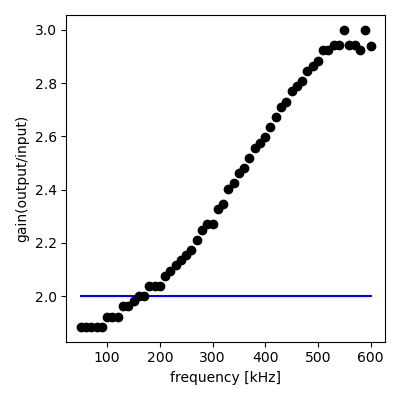
\includegraphics[width=4.3cm]{../results/preamplifier_gain_freq_plot(gain2).png}
        \caption{}
    \end{subfigure}
    \hfill
    \begin{subfigure}[b]{4.3cm}
      \centering
      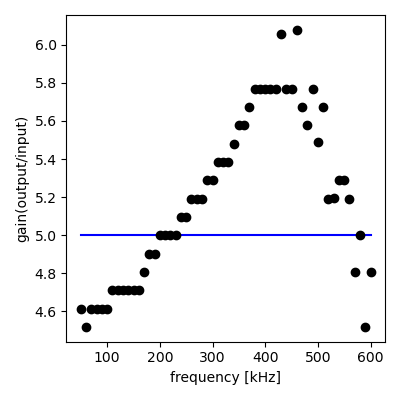
\includegraphics[width=4.3cm]{../results/preamplifier_gain_freq_plot(gain5).png}
      \caption{}
  \end{subfigure}
  \hfill
  \begin{subfigure}[b]{4.3cm}
    \centering
    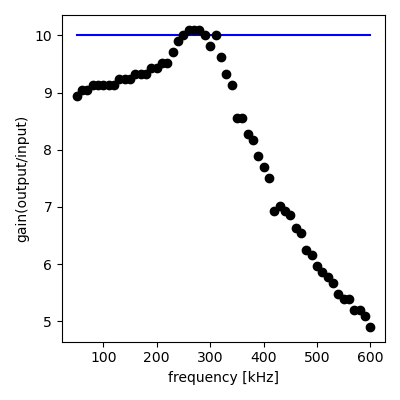
\includegraphics[width=4.3cm]{../results/preamplifier_gain_freq_plot(gain10).png}
    \caption{}
  \end{subfigure}
  \hfill
    \caption{Preamplifier Gain data for displayed gain (a) 2 (b) 5 (c) 10 in gain - frequency [$kHz$] (black dots),
     its displayed gain is in the blue line. The error bar is too small(under 1\%) to be neglected.
     }
    \label{fig: preamplifier_gain_plot}
  \end{figure}
  \begin{figure}[H]
    \begin{subfigure}[b]{4.3cm}
        \centering
        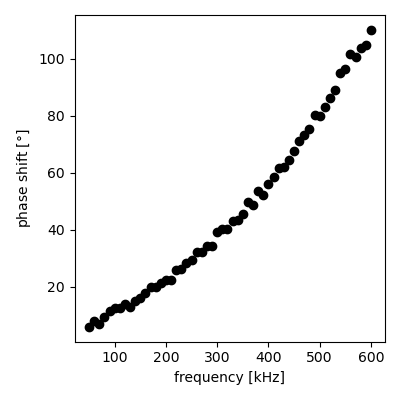
\includegraphics[width=4.3cm]{../results/preamplifier_phase_freq_plot(gain2).png}
        \caption{}
    \end{subfigure}
    \hfill
    \begin{subfigure}[b]{4.3cm}
      \centering
      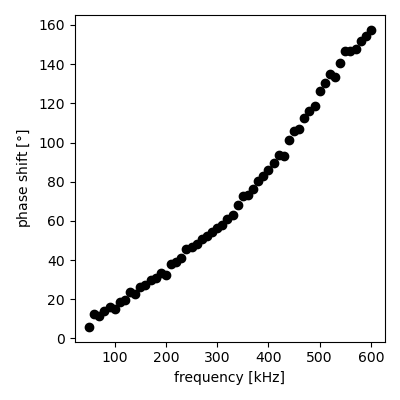
\includegraphics[width=4.3cm]{../results/preamplifier_phase_freq_plot(gain5).png}
      \caption{}
  \end{subfigure}
  \hfill
  \begin{subfigure}[b]{4.3cm}
    \centering
    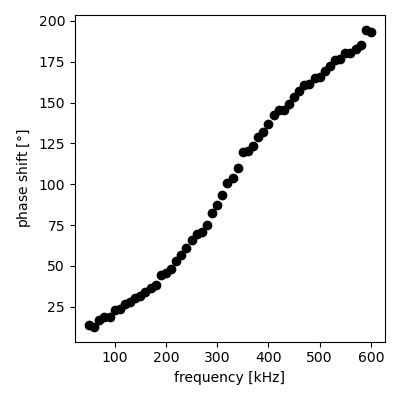
\includegraphics[width=4.3cm]{../results/preamplifier_phase_freq_plot(gain10).png}
    \caption{}
  \end{subfigure}
  \hfill
    \caption{Preamplifier phase shift data for displayed gain (a) 2 (b) 5 (c) 10 in phase[$\degree$] - frequency [$kHz$] (black dots).
    The error bar is too small(under 1\%) to be neglected.
     }
    \label{fig: preamplifier_phase_plot}
  \end{figure}

  In the log scale experiment, the 3dB frequency can be found.
  The amplified results of the frequency of $1kHz - 10MHz$ are measured, I measure several more points near 3dB frequencies.
  Fig. \ref{fig: preamplifier_loglog_plot} shows the log scale plot near 3dB frequency.
  The blue line represents the -3dB line, which highlights the -3dB position from the displayed gain.
  The red line is linear regression results near -3dB frequency.
  The specific linear regression coefficients and found -3dB frequency are listed in Fig. \ref{fig: preamplifier_statics}.
  I can find that the -3dB frequency decreases as the gain increases, which means that the filter bandwidth gets worse by increasing the gain value.
  Therefore, I use the gain value as 1 in the preamplifier module in the rest of the experiment.
  Experimentally, the real gain fits well near 1$kHz$, and even the phase shift does not found.
  But my experiment uses near 20 $Hz$ signal, the preamplifier gain and phase shift must be considered.


\begin{figure}[H]
    \begin{subfigure}[b]{4.3cm}
        \centering
        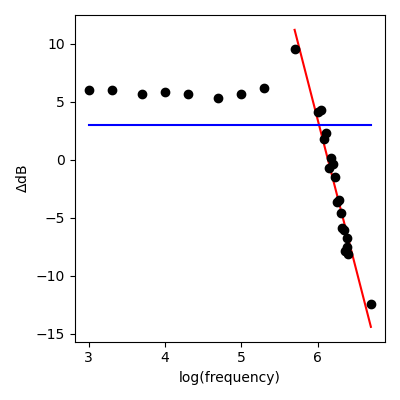
\includegraphics[width=4.3cm]{../results/preamplifier_log_plot(gain2.0).png}
        \caption{}
    \end{subfigure}
    \hfill
    \begin{subfigure}[b]{4.3cm}
      \centering
      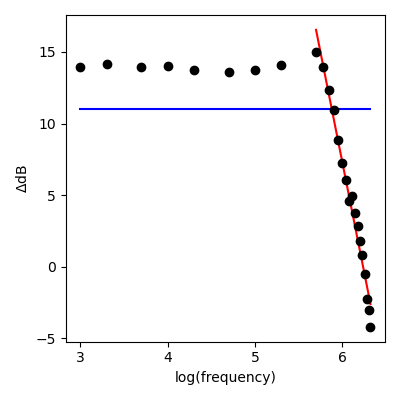
\includegraphics[width=4.3cm]{../results/preamplifier_log_plot(gain5.0).png}
      \caption{}
  \end{subfigure}
  \hfill
  \begin{subfigure}[b]{4.3cm}
    \centering
    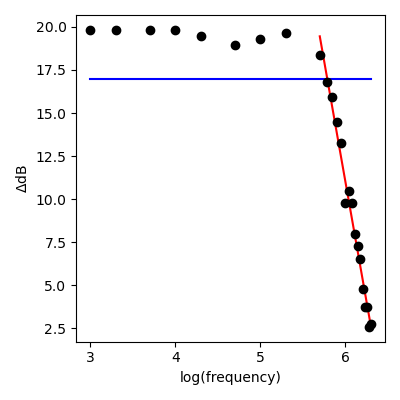
\includegraphics[width=4.3cm]{../results/preamplifier_log_plot(gain10.0).png}
    \caption{}
  \end{subfigure}
  \hfill
    \caption{Preamplifier $log(G)$ data for displayed gain (a) 2 (b) 5 (c) 10 in $\Delta dB$ - $log(f)$ (black dots),
     its -3dB line is in the blue line.
     The red line is linear regression results near -3dB frequency, the statics are given at \ref{fig: preamplifier_statics}.
     The error bar is too small(under 1\%) to be neglected.
     The $log(f)$ is in the frequency unit of [Hz]
     }
    \label{fig: preamplifier_loglog_plot}
  \end{figure}

  \begin{figure}[H]
    \centering
    \begin{tabular}{  m{2cm} | m{2.5cm} | m{2.5cm} | m{1cm}  | m{4cm}} 

      gain& a [] & b []& $R^2$ &-3dB frequency [MHz]\\ 
      \hline
        2.0 & $-26 \pm 2$& $150 \pm 47$ & 0.945& $1.04 \pm 0.11$\\
      \hline
        5.0 & $-31 \pm 1 $& $192 \pm 21$ & 0.979& $0.759 \pm 0.073$\\
      \hline
        10.0 &$ -28 \pm 1 $& $179 \pm 20$ & 0.981 & $0.612 \pm 0.052$ \\

    \end{tabular}
    \caption{
      The linear regression statics of Fig. \ref{fig: preamplifier_loglog_plot}.
      The gain stands for displayed gain in the preamplifier.
      Each coefficient is dimension-free since the plot x, and y-axis does not have one.
    }  
    \label{fig: preamplifier_statics}
\end{figure}

\subsection{Phase Shifter: Lagging phase detection}
\label{results: phase shifter}
 The phase shifter also has an unexpected phase response.
 The displayed phase shift value is controlled by two dials.
 The first dial controls the phase in a unit of $90\degree$, and the secondary fine phase dial controls the accurate proportion to the first dial.
 For example, to shift $75\degree$ the phase dial is set up to $0\degree$ and the fine phase should point out $75\degree$.
 It is experimentally sure that in fixed frequency, the total rotation of a phase dial spans $360\degree$ phase shift.
 However, the lagged phase is too definite to ignore, having a linear relationship with frequency.
 Fig. \ref{fig: phaseshifter_phase_plot} shows the frequency dependant lagged phase results.
 The red lines are linear regression results and fit very well.
 Specific regression results are given in Fig. \ref{fig: phase shifter linear regression results}.
 Also, the gain has changed in the response of the circuit.
 Fig. \ref{fig: phaseshifter_gain_plot} shows the frequency dependant gain results.
 In the ideal circuit, the gain should never change from 1.
 But the experimental results do not doubt claim the phase shifter gives an unexpected gain response.
 And it is even worse, the gain data is far above 1, and peak natured.
 The data shows there are somehow resonance phenomena near 400[$Hz$].
 There are two big meanings in these results.
 First, I can never trust the displayed phase in this group of experiments.
 Since the lagged phase extends over $180\degree$, the displayed phase shift can not be trusted.
 Moreover, the preamplifier gives meaningful phase shifts and fluctuating gain results.
 This reasoning leads me to fix the circuit to directly measure the real shifted phase in the experiment.
 I don't use the linear regression results to convert the displayed phase into the real shifted phase but to put two of the signal directly in the oscilloscope.
 Secondly, the peaked nature of the gain-frequency plot means this phase shifter circuit contains RC and an operational amplifier module inside.
 The phase shifter is usually formed based on an RC circuit.
 Contrary expectation to the ideal operational amplifier in the core of the circuit, the operational amplifier may follow Shockley's equation to ruin the frequency-independent phase shift property.
 There are no specific circuit diagrams revealed in \cite{signal_processor}, no more analysis is available.

 
 \begin{figure}[H]
    \begin{subfigure}[b]{3.1cm}
        \centering
        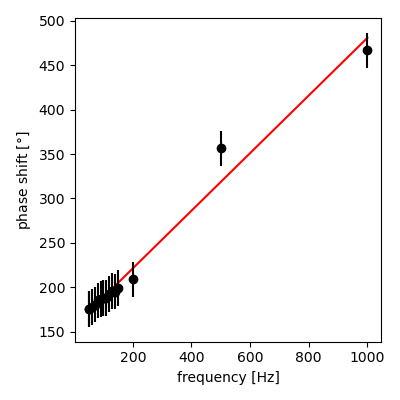
\includegraphics[width=3.1cm]{../results/phaseshifter_phase_freq_plot(phase0).png}
        \caption{}
    \end{subfigure}
    \hfill
    \begin{subfigure}[b]{3.1cm}
      \centering
      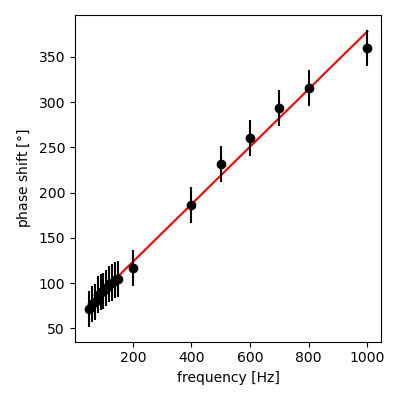
\includegraphics[width=3.1cm]{../results/phaseshifter_phase_freq_plot(phase90).png}
      \caption{}
  \end{subfigure}
  \hfill
  \begin{subfigure}[b]{3.1cm}
    \centering
    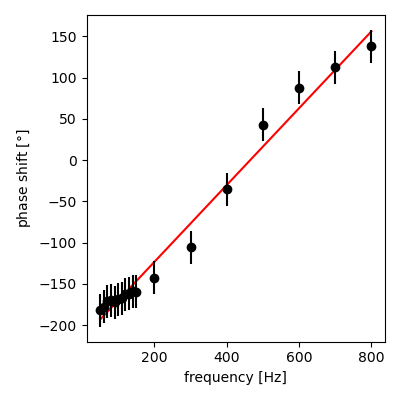
\includegraphics[width=3.1cm]{../results/phaseshifter_phase_freq_plot(phase180).png}
    \caption{}
  \end{subfigure}
  \hfill
  \begin{subfigure}[b]{3.1cm}
    \centering
    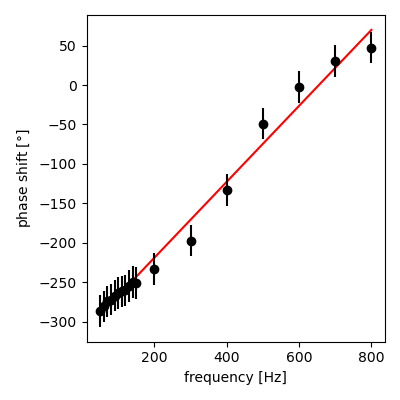
\includegraphics[width=3.1cm]{../results/phaseshifter_phase_freq_plot(phase270).png}
    \caption{}
  \end{subfigure}
  \hfill
    \caption{Phaseshifter lagged phase data for displayed phase shift (a) 0$\degree$ (b) 90$\degree$ (c) 180$\degree$ (d) 270$\degree$ in lagged phase[$\degree$] - frequency [$Hz$] (black dots)
        The error bar stands for $2\sigma = 20\degree$, the red line is linear regression results.
     }
    \label{fig: phaseshifter_phase_plot}
  \end{figure}

  \begin{figure}[H]
    \begin{tabular}{  m{3cm} | m{3cm} | m{3cm} | m{3cm}  } 

      displayed phase[$\degree$]& a[$\degree/Hz$] & b[$\degree$] & $R^2$\\ 
      \hline
        0 & $0.324 \pm 0.03 $ & $ 156 \pm 5$& 0.979\\
      \hline
        90 & $0.319 \pm 0.03$& $60 \pm 5$& 0.997\\
      \hline
      180 & $0.466 \pm 0.03$& $-217 \pm 5$& 0.983\\
      \hline
      270 & $0.481 \pm 0.03$& $-315 \pm 5$& 0.986
    \end{tabular}
    \caption{The linear regression statics of Fig. \ref{fig: phaseshifter_phase_plot}}
    \label{fig: phase shifter linear regression results}
\end{figure}

\begin{figure}[H]
  \begin{subfigure}[b]{3.1cm}
      \centering
      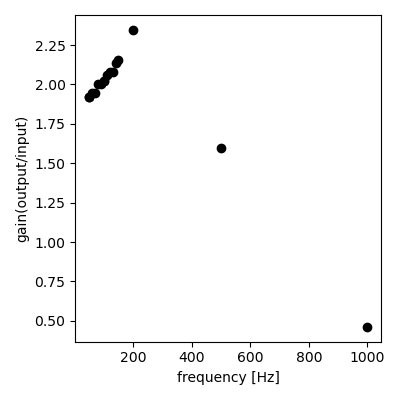
\includegraphics[width=3.1cm]{../results/phaseshifter_gain_freq_plot(phase0).png}
      \caption{}
  \end{subfigure}
  \hfill
  \begin{subfigure}[b]{3.1cm}
    \centering
    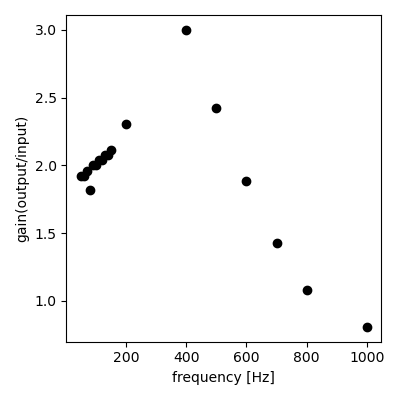
\includegraphics[width=3.1cm]{../results/phaseshifter_gain_freq_plot(phase90).png}
    \caption{}
\end{subfigure}
\hfill
\begin{subfigure}[b]{3.1cm}
  \centering
  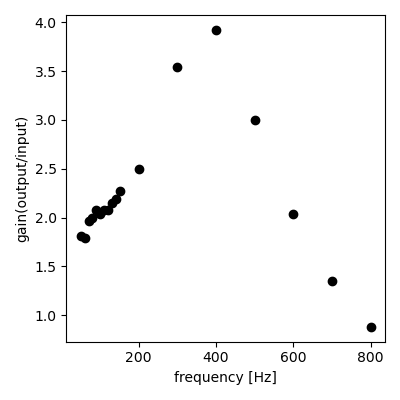
\includegraphics[width=3.1cm]{../results/phaseshifter_gain_freq_plot(phase180).png}
  \caption{}
\end{subfigure}
\hfill
\begin{subfigure}[b]{3.1cm}
  \centering
  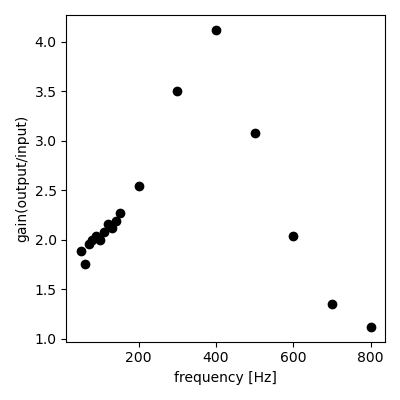
\includegraphics[width=3.1cm]{../results/phaseshifter_gain_freq_plot(phase270).png}
  \caption{}
\end{subfigure}
\hfill
  \caption{Phaseshifter gain data for displayed phase shift (a) 0$\degree$ (b) 90$\degree$ (c) 180$\degree$ (d) 270$\degree$ in gain - frequency [$Hz$] (black dots)
      The error bar is under 5\% to be disregarded.
   }
  \label{fig: phaseshifter_gain_plot}
\end{figure}


\subsection{DBM}
As mentioned at \ref{results: phase shifter}, the yellow and purple results in Fig. \ref{fig: DBM_plot} are very effective.
The phase difference between the two inputs is directly measured and intuitively matches the DBM results.
The DBM filter works very fine but, the edgy cut at the end of the wavelength has been detected.
It is because of the fluctuation of the frequencies between two inputs caused by the phase shifter, especially in low frequencies (10-100 [Hz]).
But the area of those DBM results is about a few $\mu V \cdot s$, which means those edge effects can be neglectable in the calculation of Lock-In detection.

\begin{figure}[ht]
  \begin{subfigure}[b]{6.3cm}
      \centering
      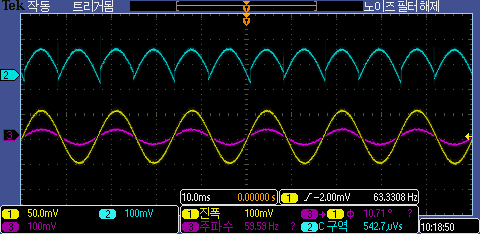
\includegraphics[width=6.3cm]{../raw_data/TEK00355.PNG}
      \caption{}
  \end{subfigure}
  \hfill
  \begin{subfigure}[b]{6.3cm}
    \centering
    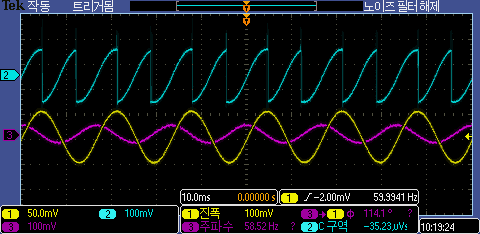
\includegraphics[width=6.3cm]{../raw_data/TEK00356.PNG}
    \caption{}
\end{subfigure}
\hfill
\begin{subfigure}[b]{6.3cm}
  \centering
  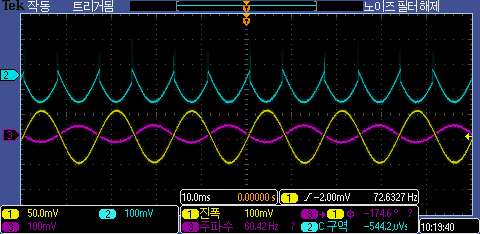
\includegraphics[width=6.3cm]{../raw_data/TEK00357.PNG}
  \caption{}
\end{subfigure}
\hfill
\begin{subfigure}[b]{6.3cm}
  \centering
  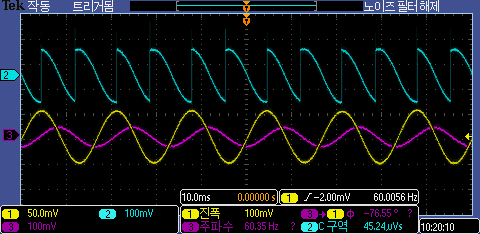
\includegraphics[width=6.3cm]{../raw_data/TEK00358.PNG}
  \caption{}
\end{subfigure}
\hfill
  \caption{DBM signal results of phase difference (a) 0 (b) 90 (c) 180 (d) 270 [$\degree$], of 50[Hz] frequency input.
      The yellow signal is the reference input voltage, and the purple one represents the phase-shifted signal.
      The blue signal is the signal after the DBM calculation.
   }
  \label{fig: DBM_plot}
\end{figure}

The measurement error of voltage is about $1mV$, and the time interval must be calculated by $1/f$.
For the null hypothesis, the DBM edge effect affects the Lock-In detection is rejected.
The phase detection error is about $5 \degree$, by the fluctuation.
The standard error of the area is $40 \mu V \cdot s$.
The experimental results are found around the standard error.



\subsection{Low Pass Filter}
\label{results: low pass filter}

 The low pass filter works with the impedance ratio of the input and output channels.
 An inductor does not help to amplify low-frequency signals, the fitting function is as follows equation \ref{equation: LPF fitting function}.
 The roll-off factor (dB/Oct) is the term that after filtering area, the amount of amplitude decay by 1 octave.
 This means, the gradient in $\log(f) - 20\log(G)$ plot value can be modified by the circuit.
 Moreover, the noise from this filter is devastating to read accurate values in the oscilloscope.
 Fig. \ref{fig: raw_plot of LPF} is the oscilloscope screenshots of 20[$Hz$] signal input, $12 dB/oct$ roll-off and 0.03 [s]-time constant.
 To find a 3dB frequency, the measurement in high-frequency signal in low pass filter is unavoidable.
 But, the noise is not neglectable in high-frequency response, I read the median value in each data in the grid.
 Some of the data in high-frequency is even unreadable, so the measurement error is about 5dB.

 \begin{figure}[H]
  \centering
  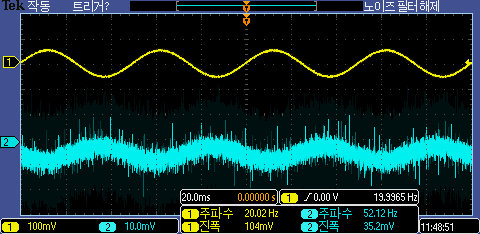
\includegraphics[width = 6cm] {../raw_data/TEK00484.PNG}
  \caption{The oscilloscope screenshots of 20[$Hz$] signal input, $12 dB/oct$ roll-off and 0.03 time constant}
  \label{fig: raw_plot of LPF}
 \end{figure}

 Fig. \ref{fig: LPF plot} shows the gain in dB to frequencies in log scale plots.
 The red line is the fitted line following equation \ref{equation: LPF fitting function}.
 The blue line is a $-3dB$ line and the intersection point with the fitted line gives 3dB frequency, the useful parameter of the filter.
 The specific results of the fitting parameter are given in Fig. \ref{fig: LPF statics}.
 The gain value has a big measurement error and dominates the statics error.
 The measured time constant has a large difference from a displayed time constant, and it is because of the dB/Oct modification module.
 To modify dB/Oct in the low pass filter, the simple fitting function as equation \ref{equation: LPF fitting function} is invalid.
 The RC circuit must contain secondary propagation of an operational amplifier, which makes the fitting function more complex than before.
 But the fact is clear and the higher time constant, the lower dB/Oct gives less 3dB frequency.
 The less 3dB frequency implies the sharp filtering performance of the low pass filter, I fixed these parameters in dB/Oct 12, time constant of 0.03 [s] in other experiments.

 \begin{equation}
  G = \frac{1}{\sqrt{(2 \pi f \tau)^2 +1}}
  \label{equation: LPF fitting function}
 \end{equation}


 \begin{figure}[H]
  \begin{tabular}{  m{3cm} | m{4cm} | m{1cm} | m{1cm} | m{3cm}  } 

    displayed dB/Oct& displayed time constant[s] & $\tau$[s] & $R^2$ & 3dB frequency [Hz]\\ \hline
     \multirow{3}{*}{6}& 0.03  & 0.06 & 0.89 & 2.7 \\ \cline{2-5}
       & 0.1& 0.33 & 0.92 & 0.49\\ \cline{2-5}
       & 0.3& 0.43 & 0.98 & 0.37\\ \hline
       \multirow{3}{*}{12}& 0.03  & 0.12 & 0.98 & 1.3 \\ \cline{2-5}
       & 0.1& 0.35 & 0.82 & 0.46\\ \cline{2-5}
       & 0.3& 0.96 & 0.88 & 0.16\\ \hline
    
  \end{tabular}
  \caption{The linear regression statics of Fig. \ref{fig: phaseshifter_phase_plot}, std error of $\tau$ and 3dB frequency are 0.03 [s], 0.2 [Hz] respectively.
  This error is from a measurement error, not a statistic error.}
  \label{fig: LPF statics}
\end{figure}

 \begin{figure}[H]
  \begin{subfigure}[b]{6.3cm}
      \centering
      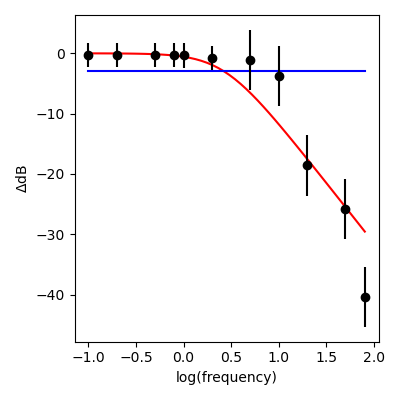
\includegraphics[width=6.3cm]{../results/low_pass_filter_gain_freq_plot(db_oct6)(time_constant0.03).png}
      \caption{}
  \end{subfigure}
  \hfill
  \begin{subfigure}[b]{6.3cm}
    \centering
    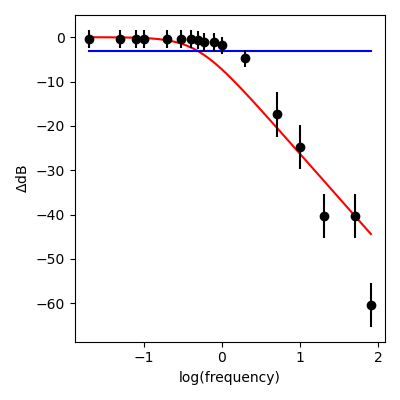
\includegraphics[width=6.3cm]{../results/low_pass_filter_gain_freq_plot(db_oct6)(time_constant0.1).png}
    \caption{}
\end{subfigure}
\hfill
\begin{subfigure}[b]{6.3cm}
  \centering
  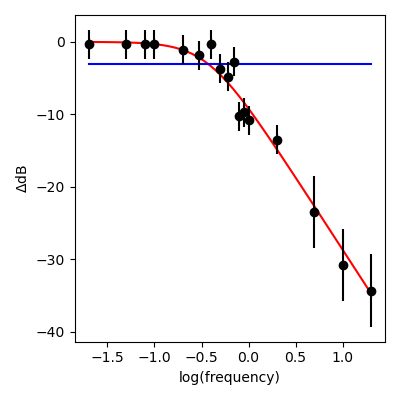
\includegraphics[width=6.3cm]{../results/low_pass_filter_gain_freq_plot(db_oct6)(time_constant0.3).png}
  \caption{}
\end{subfigure}
\hfill
\begin{subfigure}[b]{6.3cm}
  \centering
  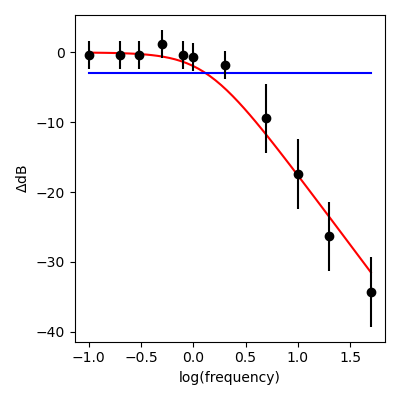
\includegraphics[width=6.3cm]{../results/low_pass_filter_gain_freq_plot(db_oct12)(time_constant0.03).png}
  \caption{}
\end{subfigure}
\hfill
\begin{subfigure}[b]{6.3cm}
  \centering
  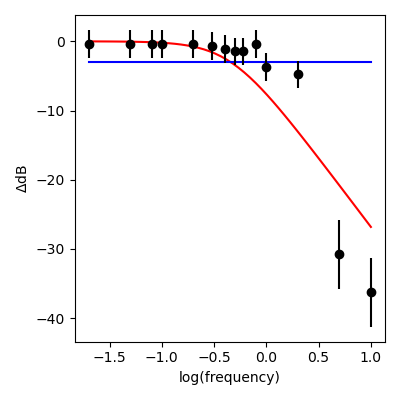
\includegraphics[width=6.3cm]{../results/low_pass_filter_gain_freq_plot(db_oct12)(time_constant0.1).png}
  \caption{}
\end{subfigure}
\hfill
\begin{subfigure}[b]{6.3cm}
  \centering
  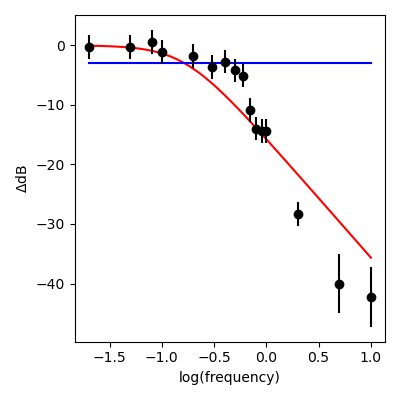
\includegraphics[width=6.3cm]{../results/low_pass_filter_gain_freq_plot(db_oct12)(time_constant0.3).png}
  \caption{}
\end{subfigure}
\hfill
  \caption{The low pass filter gain results ($20 \log G$) of dB/Oct 6, time constant (a) 0.03 (b) 0.1 (c) 0.3, dB/Oct 12, time constant (d)0.03, (e) 0.1, (f) 0.3 [$s$], in the function of $log(f)$, the black dot.
    The blue line is the $-3dB$ line and the red line is the fitted results, following equation (\ref{equation: LPF fitting function}).}
  \label{fig: LPF plot}
\end{figure}


\subsection{Lock-In Amplifier: Noise detection}
\label{results: noise detection}
 The lock-in amplifier is stable with the noise in the signal.
 To check this in experimental backgrounds, the two steps are carried out.
 First, the Fast Fourier Transform (FFT) of the signal with noise is measured in Fig. \ref{fig: noise_fft}
 As the signal-to-noise ratio (S/N) value increases, the FFT results get broadened from the frequency value of 0.
 The data shows that the FFT results in a frequency $600 [kHz]$ have the same value regarding the S/N values.
 This step checks the noise generator can make pure random noises.
 If the noise is not pure enough, there must be a repeated amplitude by a certain time.
 The certain time must leave its trace in FFT results at the high-frequency tail, which the experiment never showed.
 Therefore, the noise is random enough to examine the lock-in detection stability.
 The oscilloscope FFT results can only move its frequency in $200 [kHz]$ unit, I use $600 [kHz]$ signal frequency to check the randomness.
 The assumption is used here that, the pureness of noise generator is not related to signal frequency a lot, which is a very valid assumption.

 \begin{figure}[H]
  \begin{subfigure}[b]{6.3cm}
      \centering
      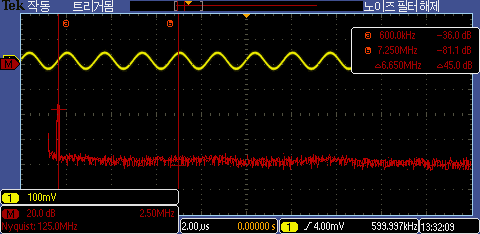
\includegraphics[width=6.3cm]{../raw_data/TEK00528.PNG}
      \caption{}
  \end{subfigure}
  \hfill
  \begin{subfigure}[b]{6.3cm}
    \centering
    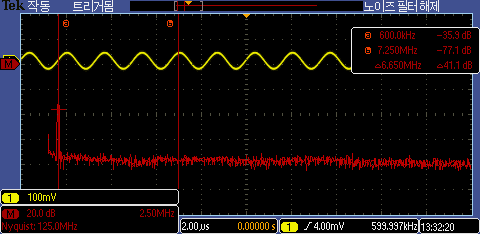
\includegraphics[width=6.3cm]{../raw_data/TEK00530.PNG}
    \caption{}
\end{subfigure}
\hfill
\begin{subfigure}[b]{6.3cm}
  \centering
  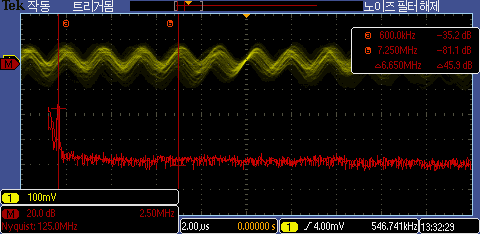
\includegraphics[width=6.3cm]{../raw_data/TEK00532.PNG}
  \caption{}
\end{subfigure}
\hfill
\begin{subfigure}[b]{6.3cm}
  \centering
  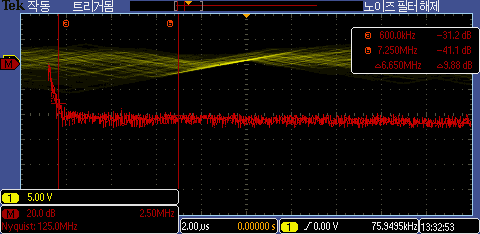
\includegraphics[width=6.3cm]{../raw_data/TEK00534.PNG}
  \caption{}
\end{subfigure}
\hfill
  \caption{FFT results in S/N ratio (a) 0 (b) $10^{-4}$ (c) $10^{-2}$ (d) $1$.
    The base signal frequency is 600 [kHz], the signal attenuator value is 1, and the gain is set to 1 in the preamplifier.
   }
  \label{fig: noise_fft}
\end{figure}

 The second step of this experiment is to prove the lock-in detection stability of signal in differing S/N values.
 I also make two input channels in the oscilloscope in reference signal and phase shifted signal to directly measure the phase difference.
 Fig. \ref{fig: lock_in_phase_plot} is the plot of signal results by phase in different S/N values.
 The plot and the data never change by the Noise amplitude, since the noise is never able to pass the lock-in detection filter.
 Fig. \ref{fig: lock_in_phase_statics} is the statics of the fitting line in Fig. \ref{fig: lock_in_phase_plot}.
 The fitting function is used a quadratic equation, $a(\phi - \phi_{max})^2 + V_0$, with high accuracy.
 The maximum voltage occurs at the phase difference in $\phi_{max}$, its value is stable by the S/N values.
 It is definite to be maximum at $\phi_{max}=0 \degree$, since the two coherent sine functions will give low-frequency signal high,
 to be filtered after the low pass filter.
 Through this experiment, it is proved that the random noise does not affect the lock-in signal at all.
 As the hall element signal is too low, the noise stability of detection is important.
 And also, if the element has a phase response, the DC-offset can reveal, which is natural but not pure noise perturbation.
 Therefore, the DC-offset stability is checked either at \ref{results: dc_offset}.


 \begin{figure}[H]
  \begin{subfigure}[b]{6.3cm}
      \centering
      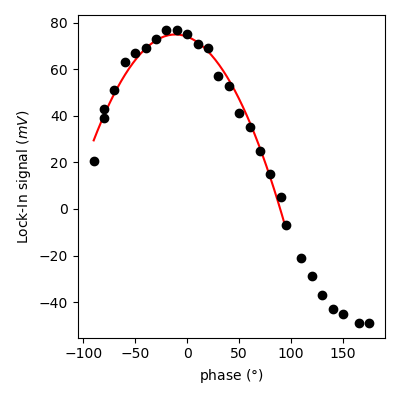
\includegraphics[width=6.3cm]{../results/lock_In_phase_plot(Noiseoff).png}
      \caption{}
  \end{subfigure}
  \hfill
  \begin{subfigure}[b]{6.3cm}
    \centering
    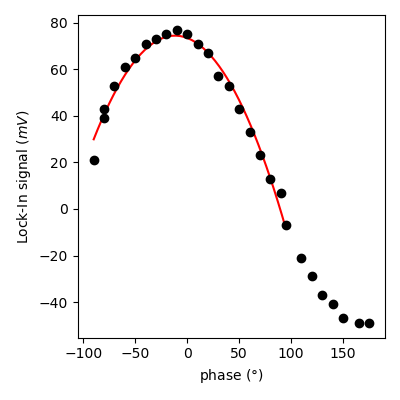
\includegraphics[width=6.3cm]{../results/lock_In_phase_plot(Noise10^-4).png}
    \caption{}
\end{subfigure}
\hfill
\begin{subfigure}[b]{6.3cm}
  \centering
  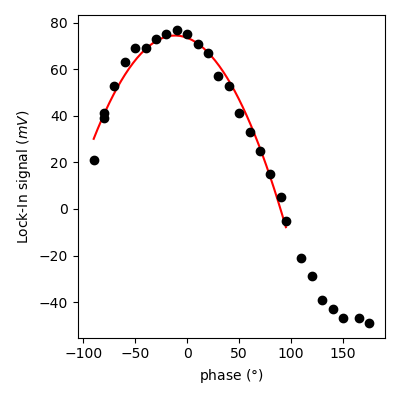
\includegraphics[width=6.3cm]{../results/lock_In_phase_plot(Noise10^-3).png}
  \caption{}
\end{subfigure}
\hfill
\begin{subfigure}[b]{6.3cm}
  \centering
  \includegraphics[width=6.3cm]{../results/lock_In_phase_plot(Noise10^-2).png}
  \caption{}
\end{subfigure}
\hfill
  \caption{Lock-In detection results in S/N ratio (a) 0 (b) $10^{-4}$ (c) $10^{-3}$ (d) $10^{-2}$.
    The base signal frequency is 20 [Hz], the dB/Oct value is 12, and the time constant value is 0.03 [s].
    S/N $10^{-5}$ plot is uploaded but not attached here.
   }
  \label{fig: lock_in_phase_plot}
\end{figure}

\begin{figure}[H]
  \centering
  \begin{tabular}{  m{1.5cm} | m{2cm} | m{5cm} | m{3cm} | m{1cm}  } 

    S/N & $\phi_{max} [\degree]$ & a [$mV/\degree^2$]& $V_0$[$mV$] & $R^2$\\ \hline
      0 & $-11 \pm 1$  & $(-7.35 \pm 0.01)\times 10^{-3}$ & $75 \pm 1$ & 0.979 \\ \hline
      $10^{-5}$ & $-12 \pm 2$& $(-7.35 \pm 0.03) \times 10^{-3}$ & $75 \pm 2$ & 0.973\\ \hline
      $10^{-4}$ & $-12 \pm 1$& $(-7.27 \pm 0.03) \times 10^{-3}$ & $74 \pm 2 $& 0.980 \\ \hline
      $10^{-3}$ & $-12 \pm 1$ & $(-7.23 \pm 0.01) \times 10^{-3} $& $74 \pm 2$ & 0.977 \\ \hline
      $10^{-2}$ & $-12 \pm 1$ & $(-7.4 \pm 0.1) \times 10^{-3}$ & $75 \pm 2$ & 0.980 \\ 
    
  \end{tabular}
  \caption{
    The quadratic regression results in Fig. \ref{fig: lock_in_phase_plot}, the red line.
    $(signal) = a \times (\phi - \phi_{max})^2  + V_0$ is the specific definition of each parameter respectively.
  }
  \label{fig: lock_in_phase_statics}
\end{figure}


\subsection{Lock-In detection: DC offset stability}
\label{results: dc_offset}
 The DC offset should be added only in the signal input.
 The phase-shifted reference input of the DBM circuit should never be affected.
 I use the preamplifier DC setting to add DC offset from the outer DC supply.
 But, the outer DC supply is not good enough to measure the DC input voltage in units of $10mV$.
 Also, the DC supply has a lot of noise signals, which might affect the result to assure stability.
 I assume that the DC supply noise is quite random so that it doesn't affect the lock-in detection results as proved at \ref{results: noise detection}.
 Moreover, it is fine not to read DC offset value in more accurate units only to prove its stability.

 Fig. \ref{fig: dc_offset_rawdata} shows the oscilloscope screenshots of a DC offset experiment.
 It should be noted that the axial graduation of the oscilloscope is modified appropriately to visualize three signals simultaneously.
 But the measurement noted below in the picture has a question mark at the end of the number.
 It is because of the noise from the DC supply, which is assumed as purely random noise.
 Therefore, the noise can not change the phase of the signal, the phase difference is checked at the beginning of the experiment.
 The visual check of the waveform also proves the assumption.
 Surely, two signals have a phase difference of $0\degree$, directly measured.

 Fig. \ref{fig: dc_offset_results} is the results of the lock-in signal in the various values of DC-offset value.
 The y-axis is enlarged enough, but the oscilloscope only detects the maximum value of the signal in units of $1mV$, the difference can not be found.
 Some values are not the same as others, but they can be disregarded since the signal input has an amplitude of $100mV$ which is very large to $2mV$, the deviation of the lock-in results.
 Through this experiment, the stability of the lock-in detection module to the DC-noise is proved.


 \begin{figure}[H]
  \begin{subfigure}[b]{6.3cm}
      \centering
      \includegraphics[width=6.3cm]{../additional_raw_data/TEK00250.png}
      \caption{}
  \end{subfigure}
  \hfill
  \begin{subfigure}[b]{6.3cm}
    \centering
    \includegraphics[width=6.3cm]{../additional_raw_data/TEK00254.png}
    \caption{}
\end{subfigure}
\hfill
\begin{subfigure}[b]{6.3cm}
  \centering
  \includegraphics[width=6.3cm]{../additional_raw_data/TEK00261.png}
  \caption{}
\end{subfigure}
\hfill
\begin{subfigure}[b]{6.3cm}
  \centering
  \includegraphics[width=6.3cm]{../additional_raw_data/TEK00266.png}
  \caption{}
\end{subfigure}
\hfill
  \caption{Lock-In detection results in different DC offset (a) 100\% (b) 500\% (c) 1000\% (d) 1500\% in phase difference $0\degree$.
    The base signal frequency is 20 [Hz], the dB/Oct value is 12, and the time constant value is 0.03 [s].
   }
   \label{fig: dc_offset_rawdata}
\end{figure}

\begin{figure}[H]
  \centering
  \includegraphics[width=6.3cm]{../results/lock_in_dc_stability.png}
  \caption{Lock-In detection results in a plot of DC offset ratio. the blue line is not fitting.
  }
  \label{fig: dc_offset_results}
\end{figure}


\subsection{Lock-In detection: Hall effect}
In the application of lock-in detection, the hall sensor from (\cite{hall_sensor}) is used to measure the magnetic dipole moment of the magnet.
To check whether the magnet acts like a magnetic dipole, a log axis plot is required.
In the equation of the magnetic field, I assumed the magnetic field is linear to the hall voltage by specification manual by (\cite{hall_sensor}).
Fig. \ref{fig: hall_effect_log_results}(a) is the adapted plot of hall voltage from the manual.
Therefore, the $B = B_max /V_max V$ equation is used in the first figure.
Fig. \ref{fig: hall_effect_log_results}(b) is the log scale plots in units of $[mm]$ and $[mT]$ each.
Linear regression has been applied in the signals that have distinct differences with default signal results.
The regression inclination of $log (B) = a log (d) + b$ equation is $a=-0.96 \pm 0.025$, which is very different from the theoretical value $-3$.
The distance between the magnet and the hall sensor is accurate in units of $0.1 [mm]$ since I put a magnet on the wooden stick at a perpendicular angle with a plastic ruler to attach its $0$ in the hall sensor.
The lock-in results are also very accurate in stability proved in different experiments.
So, I am not able to claim the magnet is acting as a point dipole.


\begin{figure}[H]
  \begin{subfigure}[b]{7.8cm}
    \centering
    \includegraphics[width=7.8cm]{../results/hall_sensor_character.png}
    \caption{}
\end{subfigure}
  \begin{subfigure}[b]{6.3cm}
    \centering
    \includegraphics[width=6.3cm]{../results/hall_effect_results_log_plot.png}
    \caption{}
\end{subfigure}

  \caption{(a) the hall sensor specification adapted by \cite{hall_sensor} (b) Lock-In detection results in a plot of DC offset ratio. the blue line is not fitting. }
  \label{fig: hall_effect_log_results}
\end{figure}

The magnetic field with volume is given as \ref{equation: magnetic field}.
$r, a,b,h, M$ is the distance between the magnet and sensor, width, length, height and the dipole moment density respectively.
This equation assumes the magnet has a uniform dipole moment, which may not be valid enough, so the width, length and height are considered as the effective value.
The equation limits to a point dipole magnetic field in the condition of $a,b,h << r$, but the experimental fitting proves the magnet is not small enough.

\begin{equation}
  B(r) = \frac{\mu_0 M}{\pi} \left[\tan^{-1}(\frac{ab}{2r \sqrt{4r^2 +a^2 + b^2}}) - \tan^{-1}(\frac{ab}{2(r+h) \sqrt{4(r+h)^2 + a^2+b^2}})\right]
  \label{equation: magnetic field}
\end{equation}

By using the fitting function of the equation, the result is plotted in Fig. \ref{fig: hall_sensor_results}.
The dipole moment density by the fitting is $M = (3.3 \pm 0.1) \times 10^7 [kg/ (mT s^2 mm^2)] = (3.3 \pm 0.1) \times 10^{16} [A/m]$ ($R^2 = 0.970$).
The result is very accurate by the lock-in detection.

\begin{figure}[H]
  \centering
  \includegraphics[width=6.3cm]{../results/hall_sensor_plot.png}

  \caption{(a) the hall sensor specification adapted by \cite{hall_sensor} (b) Lock-In detection results in a plot of DC offset ratio. the blue line is not fitting. }
  \label{fig: hall_sensor_results}
\end{figure}


\section{Summary}
 I pull off the lock-in detection experiment in the next step.
 The experiment has an unavoidable error of unexpected gain and phase response from each module.
 But by the method I claim allows the experiment to measure the real value of phase shift, the lock-in amplifier can measure the output signal with higher accuracy.
 Also. the magnetic dipole moment density of the magnet is successfully measured.
 The magnetic field has narrow nature of detection, the dipole moment gives a subtle response to capture noise.
 Therefore, the lock-in detection module is tested in several parameters such as S/N ratio, and frequencies.
 With the proven stability of lock-in detection, I can measure the result with high accuracy.
 But, my fitting in the last equation can not prove the magnetic dipole effective length, so only the dipole density can measure.
 The measurement data from different angles, the experimental results have more development potential left.


\bibliography{lock_in_ref}
\bibliographystyle{plain}
\end{document}